\chapter{Ziele}\label{kap:ziele}
Es wird ein Billardassistent entwickelt, welcher aufgrund des aktuellen Spielstands einen Stoss berechnet, der einerseits
einfach durchzuführen ist und andererseits eine optimale Ausgangslage für den nächsten Stoss bieten soll. Es gab bereits
einige Vorarbeiten \cite{project2:ziele}, wie aus dem Kapitel \ref{kap:vorarbeiten} zu entnehmen ist.

Die Ziele für diese Arbeit sind:
\begin{itemize}
    \item \textbf{Klassifikation} der Kugeln
    \item Eine effiziente gerichtete \textbf{Suche nach Stössen}
    \item Eine möglichst \textbf{realitätsnahe Simulation}
    \item Einige \textbf{Verbesserungen in der Darstellung}
    \item \textbf{Zwei Spielmodi}: \leavevmode
    \begin{itemize}
        \item \textbf{On-Demand-Modus}:
        Der Spieler kann eine Kugel oder einen Kugeltypen (Farbe) wählen, nach dem gesucht wird.
        Daraufhin werden ihm alle gefundenen Resultate in geordneter Reihenfolge nach Schwierigkeit dargestellt.
        Die Suche kann über mehrere Stösse gehen und dabei werden auch die Regeln des Spiels beachtet.
        Dies ist wichtig, um die optimale Platzierung der weissen Kugel zu eruieren.
        Nach einem Stoss kann der Spieler wiederum eine Wahl treffen.
        \item \textbf{Infinity-Modus}:
        Die Idee dahinter ist die vereinfachte Einführung des Spielers.
        So soll das System bei stabilem Zustand automatisch eine Suche nach allen Kugeln starten und das beste Ergebnis anzeigen.
        Sobald der Spieler den Stoss durchgeführt hat, wird das System wiederum automatisch eine Suche starten.
        Dadurch kann ein Spieler optimal lernen, welche Stösse einfach sind und wo eine Kugel mit welcher Geschwindigkeit
        getroffen werden muss, um das gewünschte Ergebnis zu erzielen.
    \end{itemize}
\end{itemize}

Es ist weiterhin anzumerken, dass es in erster Linie um Snooker-Billard geht. Dies hat mehrere Gründe. Einerseits soll
in dieser Arbeit nicht die Klassifikation der Kugeln im Zentrum stehen, sondern die Suche nach einem optimalen Stoss.
Es wird angenommen, dass dies mit Snooker-Kugeln einfacher ist als mit Pool-Billard-Kugeln.
Nichtsdestotrotz wird die Anwendung so abstrakt gehalten, dass sie mit wenig Aufwand
auf Pool-Billard portiert werden könnte. Dies bildet jedoch kein Ziel der Bachelor-Thesis.

\newpage

\section{Planung}
Die initiale Planung beinhaltet eine Auflistung der Tätigkeiten, deren zugewiesenen Meilensteine sowie
deren Schätzung in PT (Personen-Tage).
Jedem Arbeitspaket wird eine ID zugewiesen, welche bei der Zeiterfassung verlinkt wird.
Die ID optionaler Ziele beginnt mit einem O.
Das Total der zu vergebenden PT beträgt 90.

\begin{table}[ht]
    \rowcolors{1}{\seccolor!10}{\seccolor!10} % Rows with 10% of secondary color
    \begin{tabular}{llll}
        \rowcolor{\seccolor!50}
        ID & Name & Meilenstein & Schätzung in PT\\\bfhmidline
        T-1 & Klassifikation der Kugeln & M-1 & 6\\\bfhmidline
        T-2 & Aufsetzen Dokumentation & M-1 & 1\\\bfhmidline
        T-3 & Beschreibung Suchalgorithmus & M-1 & 3\\\bfhmidline
        T-4 & Implementation Suchalgorithmus & M-1 & 5\\\bfhmidline
        T-5 & Beschreibung der physikalischen Eigenschaften für die einfache Suche & M-1 & 6\\\bfhmidline
        T-6 & Implementation der einfachen Suche und deren Bewertungsfunktion& M-1 & 14\\\bfhmidline
        T-7 & Beschreibung der physikalischen Eigenschaften für die erweiterte Suche & M-2 & 6\\\bfhmidline
        T-8 & Implementation der erweiterten Suche und deren Bewertungsfunktion& M-2 & 8\\\bfhmidline
        T-9 & Überprüfen/Verbessern der Detektionsgenauigkeit & M-1 & 6\\\bfhmidline
        T-10 & Video erstellen & M-3 & 2\\\bfhmidline
        T-11 & Plakat schreiben & M-3 & 2\\\bfhmidline
        T-12 & Book-Eintrag schreiben & M-3 & 1\\\bfhmidline
        T-13 & Präsentation des Finaltags vorbereiten & M-3 & 2\\\bfhmidline
        T-14 & Präsentation der Verteidigung vorbereiten & M-3 & 2\\\bfhmidline
        T-15 & Finalisieren Dokumentation andere Arbeiten & M-3 & 4\\\bfhmidline
        T-16 & Projektmanagement & Kein & 4\\\bfhmidline
        T-17 & Effizienz Erfassung und Steigerung der einfachen Suche & M-1 & 0\\\bfhmidline
        T-18 & Effizienz Erfassung und Steigerung der erweiterten Suche & M-2 & 0\\\bfhmidline
        T-19 & Dokumentation der Resultate der einfachen Suche & M-1 & 6\\\bfhmidline
        T-20 & Dokumentation der Resultate der erweiterten Suche & M-2 & 2\\\bfhmidline
        T-21 & Umbau in Unity & M-1 & 4\\\bfhmidline
        T-22 & Infinity-Modus & M-1 & 5\\\bfhmidline
        O-1 & Suche über mehrere Spielstände & M-2 & \\\bfhmidline
        O-2 & Detektion des Queues in 2D & M-2 & \\\bfhmidline
        O-3 & Detektion des Queues in 3D & M-2 & \\\bfhmidline
        O-4 & Stossberechnung anhand detektiertem Queue in 2D & M-2 & \\\bfhmidline
        O-5 & Stossberechnung anhand detektiertem Queue in 3D & M-2 & \\\bfhmidline
        O-6 & Spielerabhängige Heuristik & M-2 & \\\bfhmidline
        O-7 & Live-Verfolgung und Darstellung der Kugeln & M-2 & \\\bfhmidline
        \multicolumn{3}{c}{Total} & 90\\
    \end{tabular}
    \caption{Ziele}
    \label{tab:targets}
\end{table}

\subsection{Meilensteine}
Es werden drei Meilensteine definiert, welche auch aus optionalen Zielen bestehen können. Werden diese nicht erreicht, so
gilt der Meilenstein trotzdem als erreicht. Die Deadlines ergeben sich
aus den Schätzungen der zugewiesenen Arbeitspakete.

~\\

\textit{\textbf{Meilenstein 1 - 15.11.2021}}
Das Ziel ist eine sehr einfache simple Suche. Darunter zu verstehen ist eine Lösung, welche einen direkten Treffer findet
(Weiss -> Kugel -> Loch).\\
\textit{Code Deliverables:}
\begin{description}
    \item[Klassifikation - T-1]\hfill \\
    Alle Kugeln können entsprechend ihrere Farbe klassifiziert werden.
    \item[Suchalgorithmus für einfache Suche - T-4, T-6, T-17]\hfill \\
    Ein direkter Stoss wird in akzeptabler Zeit gefunden.
    \item[Unity-Umbau - T-21]\hfill \\
    Unity ist bereit für den Einsatz.
    Zum Umbau gehören insbesondere die Farbe der Markierung der Kugeln und deren Bahnen.
    Weiterhin muss Unity mehrere Suchergebnisse anzeigen können.
    \item[Infinity-Modus - T-22]\hfill \\
    Der Spieler erhält automatisch einen Vorschlag für einen Stoss, wenn die Kugeln auf dem Tisch stillstehen.
    Sobald der Spieler einen Stoss ausgeführt hat und die Kugeln wieder stillstehen, wird der nächste Stoss vorgeschlagen.
    Vorgeschlagen werden Stösse, welche eine beliebige Kugel ins Loch spielen.
\end{description}
\textit{Dokumentation Deliverables:}
\begin{description}
    \item[Klassifikation - T-1]\hfill \\
    Das Vorgehen der Klassifikation wie deren Resultate und Genauigkeit sind dokumentiert.
    \item[Suchalgorithmus für Suche - T-3]\hfill \\
    Der Algorithmus der Suche ist theoretisch und mit Pseudocode beschrieben.
    Die theoretische Beschreibung muss nicht gänzlich mit der effektiven Implementation übereinstimmen, da diese auf
    Performance optimiert wird.
    \item[Resultate der einfachen Suche - T-19]\hfill \\
    In den Resultaten ist die Genauigkeit und Performance des einfachen Suchvorgangs
    beschrieben.
    \item[Physik der einfachen Suche - T-5]\hfill \\
    Die benötigte Physik der einfachen Suche ist beschrieben.
    \item[Bewertungsfunktion - T-6]\hfill \\
    Die Bewertungsfunktion der einfachen Suche ist dokumentiert.
\end{description}

~\\

\textit{\textbf{Meilenstein 2 - 13.12.2021}}
Das Ziel ist eine erweiterte Suche, die auch indirekte Stösse über weitere Kugeln oder Banden finden kann.
Optional sollen auch mehrere Stösse berücksichtigt werden.\\
\textit{Code Deliverables:}
\begin{description}
    \item[Suchalgorithmus für erweiterte Suche - T-8, T-18]\hfill \\
    Ein indirekter Stoss wird in akzeptabler Zeit gefunden.
    \item[Suchalgorithmus über mehrere Stösse - O-1]\hfill \\
    Es werden mehrere Spielstände bei der Suche berücksichtigt.
    \item[Queue in 2D detektieren - O-2]\hfill \\
    Der Queue wird als 2D-Objekt detektiert.
    \item[Queue in 3D detektieren - O-3]\hfill \\
    Der Queue wird mittels Tiefeninformationen der Kamera als 3D-Objekt detektiert.
    \item[Stossberechnung anhand detektiertem 2D-Queue - O-4]\hfill \\
    Der Stoss wird je nach Haltung des Queues in 2D berechnet. Es wird angenommen, dass der Queue zentral auf die
    weisse Kugel gerichtet ist.
    \item[Stossberechnung anhand detektiertem 3D-Queue - O-5]\hfill \\
    Der Stoss wird je nach Haltung des Queues in 3D berechnet. Der Queue muss nicht mehr zentral auf die weisse
    Kugel gerichtet sein.
    \item[Spielerabhängige Heuristik - O-6]\hfill \\
    Je nach Spieler kann eine andere Heuristik zur Bewertung der Stösse eingestellt werden. Durch die Unterscheidung
    können für professionelle Spieler erfolgversprechendere schwerer durchzuführende und für Anfänger
    eher leichtere Stösse gefunden werden.
    \item[Live-Verfolgung und Darstellung der Kugeln - O-7]\hfill \\
    Die Kugeln werden ohne Benutzereingabe in Echtzeit getrackt und deren Position über den Projektor dargestellt.
\end{description}
\textit{Dokumentation Deliverables:}
\begin{description}
    \item[Physik der erweiterten Suche - T-7]\hfill \\
    Die benötigte Physik der erweiterten Suche ist beschrieben.
    \item[Resultate der erweiterten Suche - T-20]\hfill \\
    In den Resultaten ist die Genauigkeit und Performance des erweiterten Suchvorgangs
    beschrieben.
    \item[Bewertungsfunktion - T-8]\hfill \\
    Die Bewertungsfunktion der erweiterten Suche ist dokumentiert.
\end{description}

~\\

\textit{\textbf{Meilenstein 3 - 17.01.2022}}
Das Ziel ist der Abschluss aller Arbeiten zu denen auch Plakat, Book-Eintrag oder Video gehören.\\
\textit{Deliverables:}
\begin{description}
    \item[Video - T-10]\hfill \\
    Das finale Video ist erstellt.
    \item[Plakat - T-11]\hfill \\
    Das Plakat ist erstellt.
    \item[Book-Eintrag - T-12]\hfill \\
    Der Book-Eintrag ist erstellt.
    \item[Präsentation für Finaltag - T-13]\hfill \\
    Die Präsentation/Ausstellung für den Finaltag ist vorbereitet.
    \item[Präsentation für Verteidigung - T-14]\hfill \\
    Die Präsentation für die Verteidigung ist vorbereitet.
    \item[Finalisieren der Arbeiten - T-15]\hfill \\
    Die Dokumentation wie auch der Code sind abgeschlossen.
\end{description}

\newpage
\section{Risikoanalyse}
Es gibt diverse Risiken, die während dieser Arbeit eintreten können. Um das Bewusstsein dafür zu stärken,
wird vorgängig eine Risikoanalyse durchgeführt, wobei es um die Identifikation wie auch die Zuordnung deren
Auftretenswahrscheinlichkeit und Auswirkungen geht. Weiterhin werden geeignete Massnahmen definiert, die entweder
die Eintrittswahrscheinlichkeit reduziert oder bei Auftreten angegangen werden können.

Die Risiken werden im Detail aufgelistet. Die Spalte \glqq WK\grqq steht für die Eintrittswahrscheinlichkeit, welche
in den Wahrscheinlichkeiten \glqq Gering\grqq, \glqq Möglich\grqq, \glqq Wahrscheinlich\grqq, \glqq Sehr Wahrscheinlich\grqq{}
angegeben wird. Die Spalte \glqq AW\grqq{} steht für die Auswirkungen, welche in den Grössen \glqq Klein\grqq, \glqq Mittel\grqq, \glqq Gross\grqq{}
angegeben wird.

\begin{table}[ht]
    \rowcolors{1}{\seccolor!10}{\seccolor!10} % Rows with 10% of secondary color
    \begin{tabularx}{\linewidth}{llXll}
        \rowcolor{\seccolor!50}
        ID & Risiko & Massnahme & WK & AW\\\bfhmidline

        R-1 & Verlust von Programm-Sourcen & Führen eines Repositories auf GIT, welches das Wiederherstellen
        eines bestimmten Standes erlaubt. Zudem wird jeden Freitag
        ein Backup des GIT-Standes auf eine externe Festplatte
        geschrieben, sollte der unwahrscheinliche Fall eintreten, dass
        GIT nicht mehr verfügbar sein sollte oder seine Bestände verliert. & Möglich & Mittel\\\bfhmidline

        R-2 & Ausfall der Arbeitsgeräte & Es stehen Ersatzgeräte bereit, welche sofort zum Einsatz
        kommen könnten. & Möglich & Klein\\\bfhmidline

        R-3 & Krankheitsausfall der Teammitglieder & Es wird wenn möglich von Zuhause aus gearbeitet,
        um das Risiko einer Ansteckung zu vermindern. & Möglich & Gross\\\bfhmidline

        R-4 & Parallele Entwicklung derselben Funktionen & Durch eine anfängliche Planung der Arbeitspakete, wie
        auch den ständigen Austausch und Einsatz von
        Pair-Programming an geeigneten Stellen, wird
        das Risiko stark reduziert. Sollte es trotzdem
        Eintreten, sind die Auswirkungen marginal, da die
        ständige Kommunikation dies sofort aufdecken würde. & Gering & Klein\\\bfhmidline

        R-5 & Unterschätzen der Komplexität & Um zumindest ein brauchbares Resultat vorweisen zu können,
        wurde der erste Meilenstein möglichst simpel gehalten. & Wahrscheinlich & Gross\\\bfhmidline

        R-6 & Verpassen wichtiger Termine & Es wird ein Kalender mit allen Terminen geführt, welcher mehrmals eine
        Erinnerung anzeigt.& Gering & Gross\\\bfhmidline
    \end{tabularx}
    \caption{Risiken}
    \label{tab:risiken}
\end{table}

Die identifizierten Risiken werden in der Abbildung \ref{fig:risikoanalyse} für eine bessere Übersicht eingetragen.
\begin{figure}[h!]
    \begin{center}
        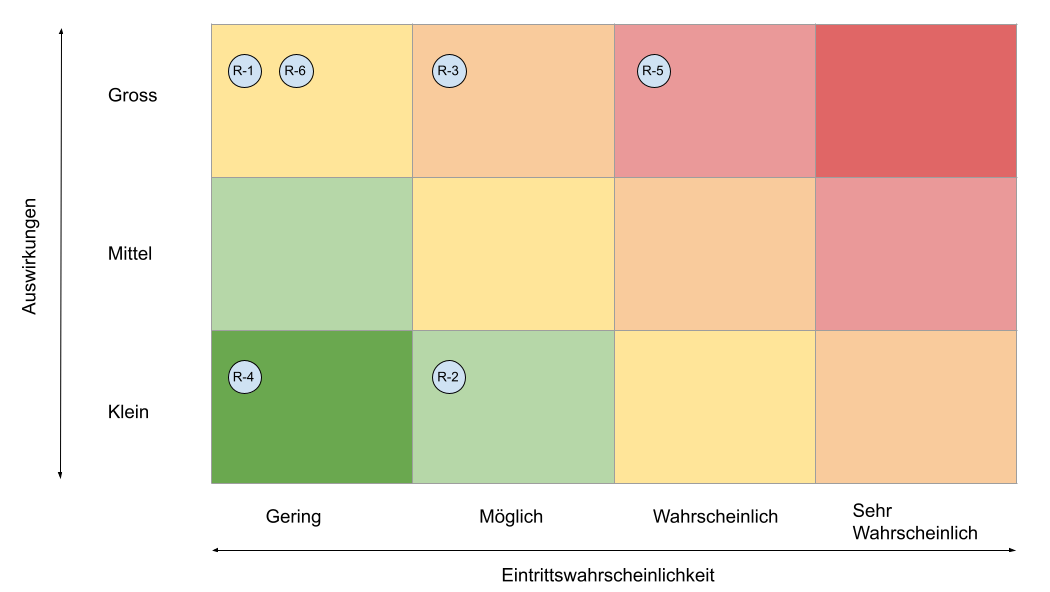
\includegraphics[width=0.8\linewidth]{../common/03_billiard_ai/resources/16_risikoanalyse.png}
    \end{center}
    \caption{Risikoanalyse}
    \label{fig:risikoanalyse}
\end{figure}
